% Hier bitte ausfüllen:
\newcommand{\praktikum}{} % Praktikum
\newcommand{\semester}{} % Semester
\newcommand{\wochentag}{} % Wochentag-Gruppe
\newcommand{\gruppennummer}{} % Gruppennummer
\newcommand{\nachnameeins}{} % Nachname1
\newcommand{\nachnamezwei}{} % Nachname2
\newcommand{\vornameeins}{} % Vorname1
\newcommand{\vornamezwei}{} % Vorname2
\newcommand{\email}{} % E-Mail Adressen
\newcommand{\versuch}{} % Versuch
\newcommand{\fehlerrechnung}{} % Fehlerrechnung
\newcommand{\betreuer}{} % Betreuer:in
\newcommand{\durchfuehrungsdatum}{} % Durchgeführt am
\newcommand{\abgabedatumeins}{} % 1. Abgabe am:
\newcommand{\abgabedatumzwei}{} % 2. Abgabe am:
%%%%%%%%%%%%%%%%%%%%%%%%%%%%%%%%%%%%%%%%%%%%%%%%%%%%%%%%%%%%%%%%%%%%%%%%%%%%%%%%%%%%%%%%%
\begin{tikzpicture}[remember picture,overlay]
    \node at (current page.center) {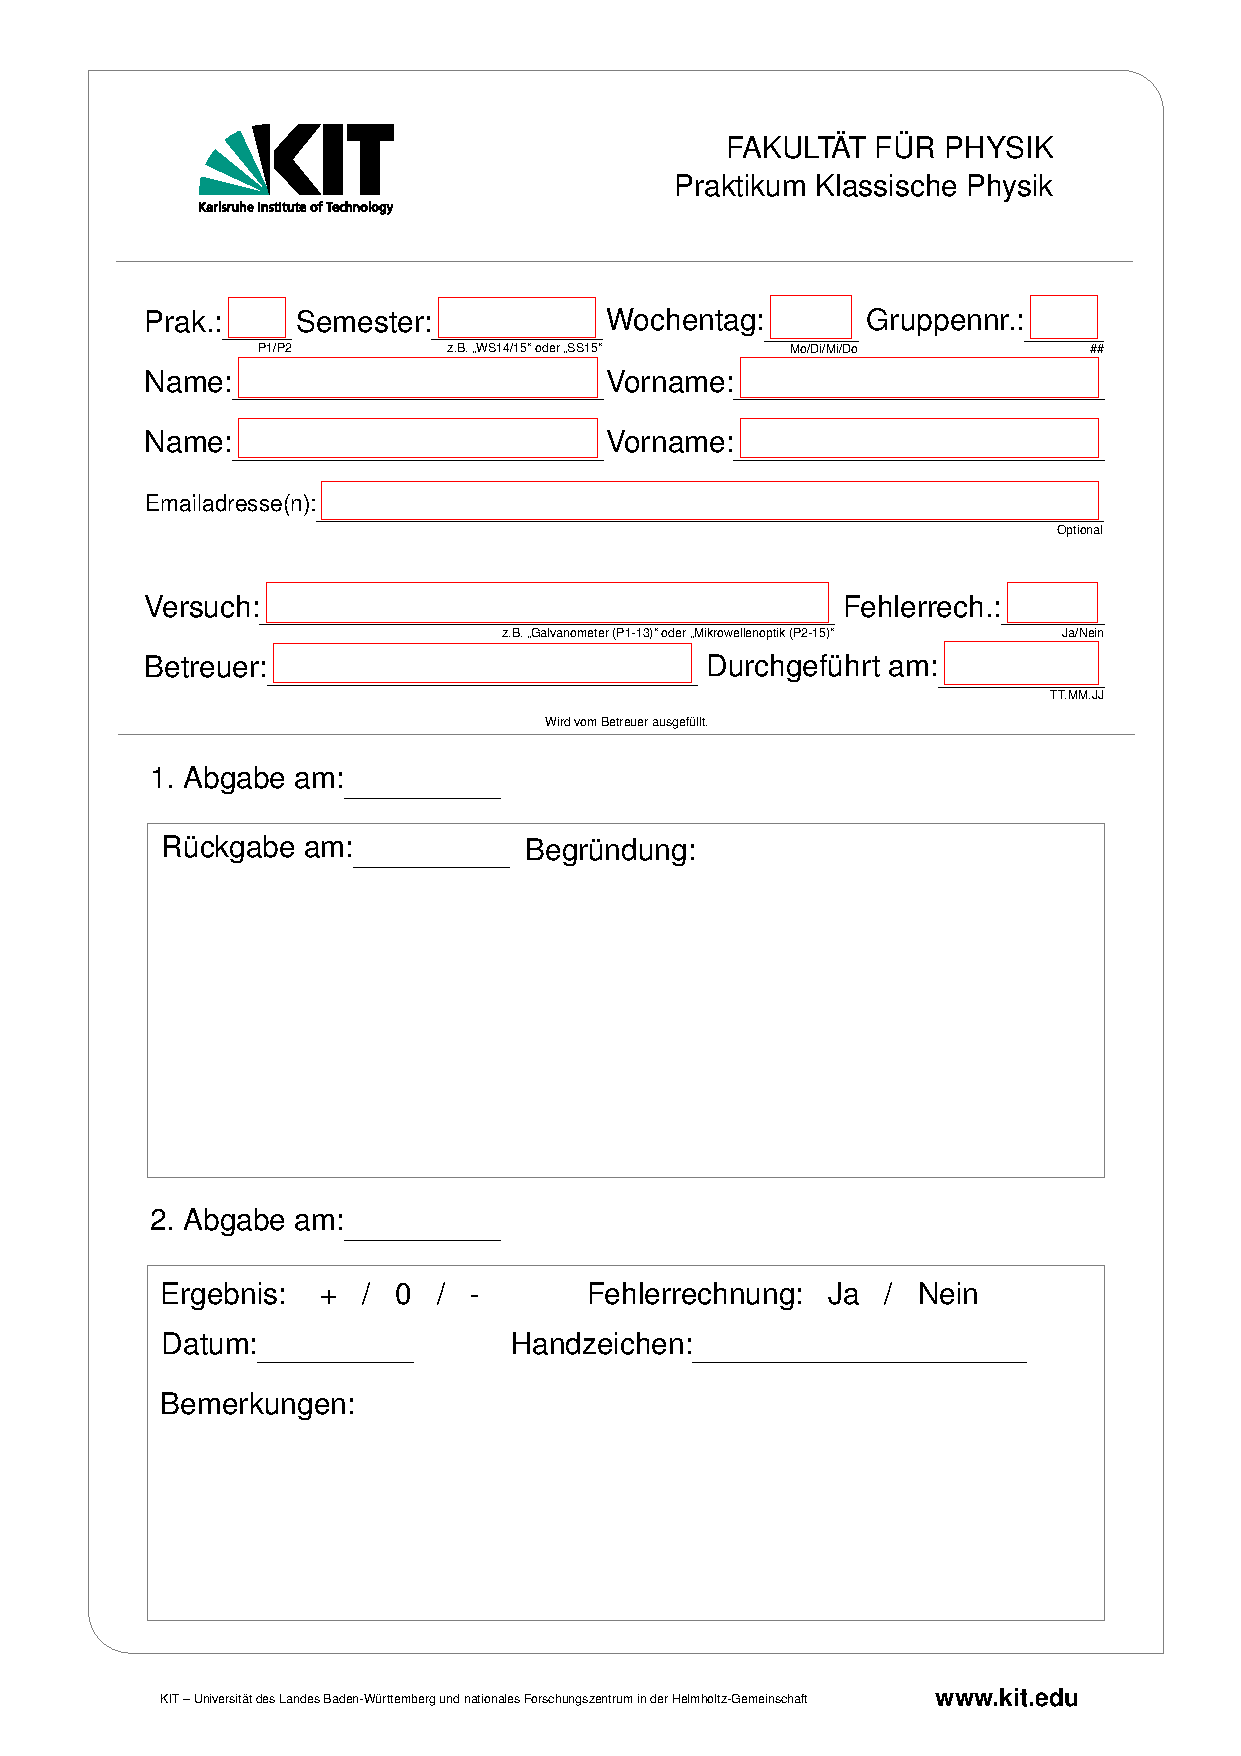
\includegraphics[page=1]{include/DeckblattP1P2.pdf}};
    \begin{scope}[shift={(current page.south west)},every node/.style={anchor=base west}]
        % Grid to help find the positions (remove in final version)
        %\draw [help lines] (0,0) grid (current page.north east);
        %\draw [help lines,thick] (0,0) grid [step=5cm] (current page.north east);
        %
        \node at (3.95cm,24.15cm) {\Large{\praktikum}}; % Praktikum:
        \node at (7.5cm,24.15cm) {\Large{\semester}}; % Semester:
        \node at (13.2cm,24.15cm){\Large{\wochentag}}; % Wochentag-Gruppe:
        \node at (17.6cm,24.15cm){\Large{\gruppennummer}};% Gruppennummer:
        \node at (4cm,23.1cm){\Large{\nachnameeins}}; % Nachname1:
        \node at (4cm,22.1cm){\Large{\nachnamezwei}}; % Nachname2:
        \node at (12.5cm,23.1cm){\Large{\vornameeins}}; % Vorname1:
        \node at (12.5cm,22.1cm){\Large{\vornamezwei}}; % Vorname2:
        \node at (5.4cm,21.1cm){\Large{\email}}; % E-Mail Adressen:
        \node at (4.5cm,19.3cm){\Large{\versuch}}; %Versuch:
        \node at (17.1cm,19.3cm){\Large{\fehlerrechnung}}; % Fehlerrechnung:
        \node at (4.55cm,18.3cm){\Large{\betreuer}}; % Betreuer:in:
        \node at (16cm,18.3cm){\Large{\durchfuehrungsdatum}}; % Durchgeführt am:
        \node at (5.9cm,16.4cm){\Large{\abgabedatumeins}}; % 1. Abgabe am:
        \node at (6cm,15.2cm){\Large{}}; %Rückgabe am:
        \node at (5.8cm,8.9cm){\Large{\abgabedatumzwei}}; % 2. Abgabe am:
    \end{scope}
\end{tikzpicture}
% This information will appear embed into the PDF file as meta data
\hypersetup{
  pdftitle    = {\praktikum\hspace{0.2222em}Protokoll - \versuch},
  pdfsubject  = {Protokoll des Versuchs \versuch\hspace{0.2222em}vom \durchfuehrungsdatum},
  pdfauthor   = {\vornameeins\hspace{0.2222em}\nachnameeins\hspace{0.2222em}und\hspace{0.2222em}\vornamezwei\hspace{0.2222em}\nachnamezwei\hspace{0.2222em}(Gruppe \wochentag\gruppennummer)},
  pdfkeywords = {KIT, Physik, Praktikum, Protokoll, \praktikum, \versuch, \semester, \vornameeins\hspace{0.2222em}\nachnameeins, \vornamezwei\hspace{0.2222em}\nachnamezwei} ,
  pdfcreator  = {pdflatex},
  pdfproducer = {LaTeX with hyperref}
}